\documentclass{article}

\usepackage[utf8]{inputenc}
\usepackage[T1]{fontenc}      
\usepackage[francais]{babel}
\usepackage{graphicx}
\usepackage{circuitikz}
\usepackage[squaren, Gray]{SIunits}
\usepackage{sistyle}
\usepackage[autolanguage]{numprint}
\usepackage{pgfplots}
\pgfplotsset{compat=1.9}
\usepackage{amsmath,amssymb,array}
\usepackage[top=2.5cm,bottom=2.5cm,right=2.5cm,left=2.5cm]{geometry}
\usepackage{url} 
\usepackage{tabularx}
\DeclareMathOperator{\dist}{d}
\newenvironment{abstract-fr}
{
	\begin{center}
		\textbf{Résumé} \\[0.5cm]
	\end{center}
}
{}

\newenvironment{abstract-en}
{
	\begin{center}
		\textbf{Summary} \\[0.5cm]
	\end{center}
}
{}
% New command pour la modélisation mécanique, tri à effectuer
\newcommand\fv[1]{{\bf #1}} % free vector
\newcommand\fvd[1]{\dot{\bf #1}} % free vector derivated
\newcommand\fvdd[1]{\ddot{\bf #1}} % free vector derivated
\newcommand\fvr[1]{\mathring{\bf #1}} % free vector relatively derivated
\newcommand\fvrr[1]{\overset{\circ\circ}{\bf #1}} % free vector relatively derivated
\newcommand\uv[1]{{\bf\hat{ #1}}} % unit vector
\newcommand\ui{{\bf\hat{I}}} % unit vector I
\newcommand\uj{{\bf\hat{J}}} % unit vector J
\newcommand\uk{{\bf\hat{K}}} % unit vector K
\newcommand\wrt[2]{\ensuremath{\tensor*[_{ #1}]{ #2}{}}} % With Respect To
\newcommand\wtr[3]{\ensuremath{\tensor*[_{ #1}]{ #2}{^{ #3}}}} % With Two Respect
\newcommand\omegaf{{\bm \omega}}
\newcommand\omegafr{\mathring{\bm \omega}}
\newcommand\omegafd{\dot{\bm \omega}}
\newcommand\omegaft{\tilde{\bm \omega}}
\newcommand\omegaftr{\mathring{\tilde{\bm \omega}}}
\newcommand\omegat{\tilde{\omega}}
\newcommand\omegatd{\tilde{\dot{\omega}}}
\newcommand\ine{{\bf I}}
\newcommand\st{{\bf L}}
\newcommand\pst{{\bf M}}
\newcommand\lm{{\bf N}}
\newcommand\am{{\bf H}}
\newcommand\amd{\dot{\am}}
\newcommand\fo{{\bf F}}
\newcommand\po{\mathcal{P}}
\newcommand\xg{\ensuremath{\fv{R}}}
\newcommand\xgd{\ensuremath{\fvd{R}}}
\newcommand\xgdd{\ensuremath{\fvdd{R}}}
\newcommand\dvec[1]{\dot{\vec{ #1}}}
\newcommand\ddvec[1]{\ddot{\vec{ #1}}}
\newcommand\qp{\dot{q}}
\newcommand\dqp{\Delta \dot{q}}
\usepackage{url} 
\usepackage{hyperref}
\hypersetup{
    colorlinks,
    citecolor=black,
    filecolor=black,
    linkcolor=black,
    urlcolor=black
}

\begin{document}

\section{Analyse séquentielle du circuit}
Dans cette section, nous allons décrire le fonctionnement du circuit
de notre haut-parleur de la manière la plus précise et la plus complète
possible. 

Cette section est découpée en quatre sections, une pour chaque bloc 
principal du circuit. Chaque bloc est associé à un rôle bien précis du
haut-parleur.

\paragraph{Remarque}
Dans cette section, la figure associé à chaque composant sera constituée
d'un schéma de ce composant à gauche et d'une photo de ce composant à droite.

\subsection{La connexion avec la prise Jack}

\begin{figure}[!hbt]
	\centering
	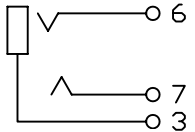
\includegraphics[scale=0.6]{jack-female.png}
	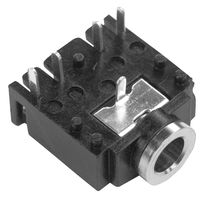
\includegraphics[scale=0.24]{jack-female-r.jpg}
	\caption{Premier bloc du circuit :
					la prise Jack femelle. (Source : datasheet du composant sur Farnell.com)}
	\label{jack-female}
\end{figure}

Ce premier bloc (Figure \ref{jack-female}), chargé de faire la connexion 
entre la source (smartphone, iPod, etc) et le reste du circuit, est constitué de la prise Jack femelle. 
Pour bien comprendre son fonctionnement, regardons d'abord à quoi ressemble la prise Jack
mâle avec laquelle elle sera couplée (Figure \ref{jack-plug}).

\begin{figure}[!hbt]
	\centering
	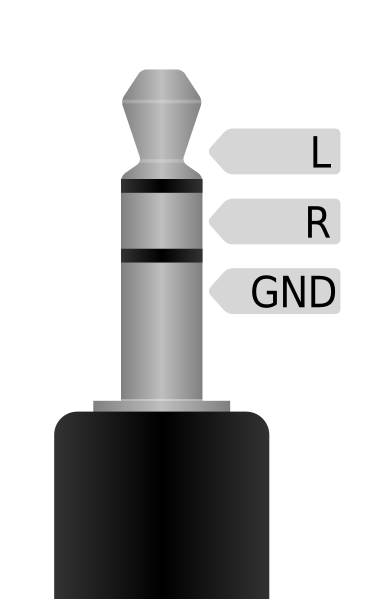
\includegraphics[scale=0.1]{jack-plug.png}
	\caption{Prise Jack mâle \unit{3.5}{\milli\meter}, contact en 3 points. (Source : Wikipédia)}
	\label{jack-plug}
\end{figure}

Cette prise Jack mâle sert à transporter un signal stéréophonique, qui sépare le 
canal gauche et le canal droit. Le canal gauche correspond à la pointe de la prise 
(L sur la figure), le canal droit correspond à l'anneau de la prise (R sur la figure). 
Le manchon de la prise correspond quant à lui à la masse.

Sur le schéma de la prise Jack femelle (Figure \ref{jack-female}), nous pouvons alors
voir que le signal du canal droit sortira du point \numprint{6}, tandis que le signal du 
canal gauche sortira du point \numprint{7}. La terre est quant à elle reliée au point
\numprint{3}. Sur le dessin de la plaquette (Figure \ref{dessin-pcb}), on remarque alors
que c'est le signal du canal droit qui sera traité par la plaquette, celui-ci se dirigeant vers
le point \textit{IN1}. Le canal gauche, dirigé quant à lui vers le point \textit{IN2} pourrait
être récupéré et dirigé vers une deuxième plaquette afin que nos deux haut-parleurs soient en stéréo.

\begin{figure}[!hbt]
	\centering
	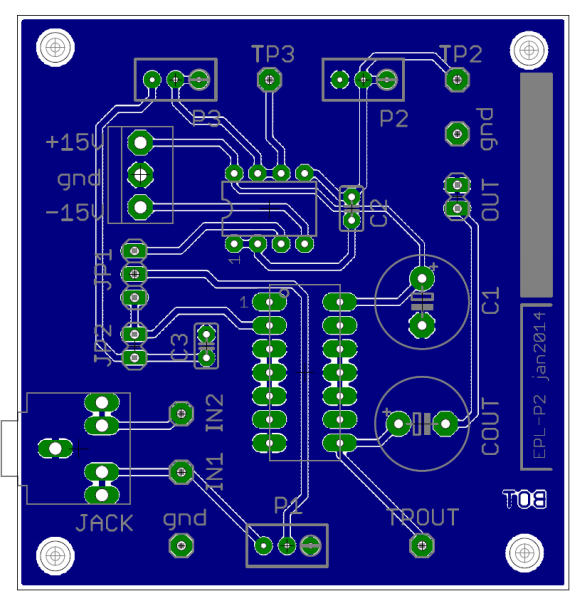
\includegraphics[scale=0.5]{dessin-pcb.png}
	\caption{Dessin de la face avant du circuit imprimé. (Source : Composants pour le projet P2, iCampus)}
	\label{dessin-pcb}
\end{figure}

\subsection{Le réglage du volume}
Le fonctionnement de ce bloc est relativement simple à comprendre, il est constitué d'un potentiomètre 
(P1 sur la Figure \ref{dessin-pcb}), c'est-à-dire d'une résistance variable.
Selon la valeur de la résistance, par la loi d'Ohm, l'amplitude du signal
sera plus ou moins réduite et donc le volume sera plus ou moins grand.

\begin{figure}[!hbt]
	\centering
	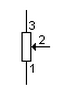
\includegraphics[scale=1.1]{pot.png}
	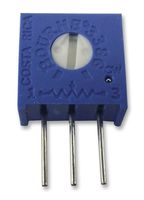
\includegraphics[scale=0.30]{pot-r.jpg}
	\caption{Potentiomètre. (Soure : datasheet du composant sur Farnell.com)}
	\label{bloc2}
\end{figure}

Nous disposions de 3 potentiomètres pour réaliser notre haut-parleur, possédant
tous une résistance maximale différente :

\begin{center}
	\begin{tabular}{l|r}
	3386W-1-101-LF & \unit{100}{\ohm} \\
	3386W-1-102-LF & \unit{1000}{\ohm} \\
	3386W-1-103-LF & \unit{10000}{\ohm} 
	\end{tabular}
\end{center}

% A verifier
Afin de permettre une plus grande variation du volume, nous avons décidé d'utiliser
le potentiomètre avec la plus grande résistance maximale en \textit{P1}.

\subsection{Le réglage des graves et des aigus}
Ce bloc-ci est sans aucun doute le plus compliqué à comprendre. Il est constitué d'un 
filtre passe-haut (réglage des aigus) et d'un filtre passe-bas (réglage des graves).
Le filtre passe-haut est celui qui suit le premier amplificateur (\textit{LM358N-A}),
le passe-bas est celui qui suit le deuxième amplificateur (\textit{LM358N-B}). 
La combinaison des deux filtres forme un filtre passe-bande, représenté sur la
Figure \ref{filtre}. 

\begin{figure}[!hbt]
	\centering
	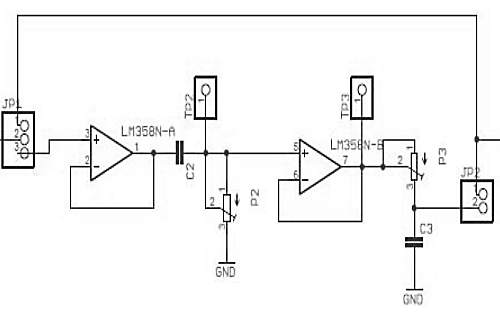
\includegraphics[scale=0.6]{filtre-passe-bande.png}
	\caption{Schéma électrique du filtre passe-bande de notre haut-parleur.
	(Source : Composants pour le projet P2, iCampus)}
	\label{filtre}
\end{figure}

Ce bloc est un petit peu plus compliqué à situer sur la Figure
\ref{dessin-pcb} car les deux amplificateurs sont situés dans le Dual ampli-op (LM358N) 
représenté à la Figure \ref{dual-ampli-op}. 

\begin{figure}[!hbt]
	\centering
	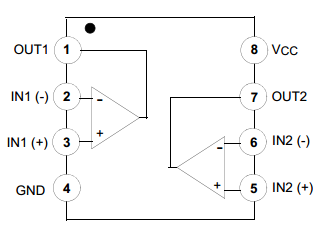
\includegraphics[scale=0.6]{dual-opamp.png}
	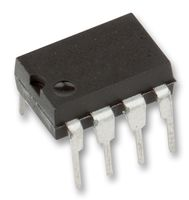
\includegraphics[scale=0.45]{dual-opamp-r.jpg}
	\caption{Le dual op-amp. (Source : datasheet du composant sur Farnell.com)}
	\label{dual-ampli-op}
\end{figure}

Ce dual ampli-op est alimenté en $\unit{\pm15}{\volt}$ par l'intermédiaire
d'un bornier.

Un autre point intéressant à relever sur le schéma du filtre est la présence d'une boucle 
reliant la sortie à la borne négative de chaque amplificateur. Ces boucles sont appelées
"boucles de contre-réaction".  Le gain normal d'un amplificateur est de l'ordre de $10^{6}$. 
Grâce aux boucles de contre-réaction, on peut contrôler le gain d'un amplificateur. 
Dans notre cas, le gain de l'amplificateur est ramené à $1$. 
Les deux amplificateurs sont ce qu'on appelle des \textit{suiveurs de tensions}. 
Leur rôle est de permettre le règlage des graves et des aigus de manière indépendante.
Sans ces amplificateurs suiveurs, faire varier le potentiomètre \textit{P2} influencerait 
non seulement le filtre passe-haut, mais influencerait aussi le filtre passe-bas 
(car les potentiomètres \textit{P2} et \textit{P3} sont en série).

Chaque filtre (passe-haut et passe-bas) est composé d'un potentiomètre et d'une capacité céramique
(Figure \ref{capac-r}) de \unit{470}{\nano\farad}.

\begin{figure}[!htb]
	\centering
	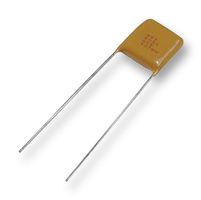
\includegraphics[scale=0.4]{capac-r.jpg}
	\caption{Capacité céramique utilisée dans les filtres. (Source : datasheet du composant sur Farnell.com)}
	\label{capac-r}
\end{figure}

% VERIFÉ
Afin d'assurer à notre haut-parleur la plus grande bande passante, nous avons utilisé le potentiomètre
dont la résistance maximale est de \unit{1000}{\ohm}) pour le filtre passe-haut et
l'autre (dont la résistance maximale est de \unit{100}{\ohm}) pour le filtre passe-bas. En effet, soient
$f_1$ et $f_2$ les fréquences de coupures respectives des filtres passe-haut et passe-bas, la norme de la 
bande passante est donnée par :

$$f_2 - f_1$$

Pour avoir la plus grande bande passante, il faut donc :

$$f_1 < f_2 \Rightarrow \frac{1}{2\pi R_1C} < \frac{1}{2\pi R_2C} \Rightarrow R_2 < R_1$$

Le choix inverse aurait pu aboutir à une bande passante nulle.

Concernant le câble reliant les points 1 du Jumper 1 (\textit{JP1}) et du Jumper 2 (\textit{JP2}), 
il s'agit en quelque sorte d'un câble de "sécurité" que l'on peut connecter afin que le signal 
ne passe pas par les filtres passe-haut et passe-bas. 
Cela pourrait nous être utile pour tester notre haut-parleur dans l'hypothèse où un des filtres 
ne fonctionnerait pas.

Enfin, nous pouvons aussi remarquer une boucle qui relie le point 1 du potentiomètre 3 (\textit{P3})
au reste du circuit. Cette boucle a simplement pour but d'éviter de laisser un câble "`dans le vide"',
et donc d'éviter les signaux parasites.

\subsection{L'amplificateur de puissance}

\begin{figure}[!htb]
	\centering
	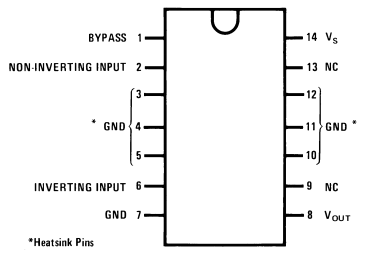
\includegraphics[scale=0.48]{ampli-audio.png}
	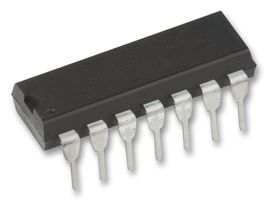
\includegraphics[scale=0.35]{ampli-audio-r.jpg}
	\caption{L'amplificateur de puissance. (Source : datasheet du composant sur Farnell.com)}
	\label{ampli-audio}
\end{figure}

Cette partie contient l'amplificateur de puissance (aussi appelé amplificateur audio). 
Cet amplificateur a pour but d'amplifier un signal électrique audio pour
permettre le fonctionnement d'un haut-parleur ou d'une enceinte acoustique.

Le nom amplificateur de puissance peut induire en erreur. En effet, comme tout amplificateur,
l'amplificateur de puissance agit sur la tension mais son impédance de sortie étant très faible,
il peut délivrer une grande puissance (ce qui lui vaut son nom).

Dans notre cas, l'amplificateur a un gain en tension de \numprint{50} et une puissance de $\unit
{2.5}{\watt}$.
% A vérifier pour la puissance, la liste des composants laisse penser qu'il s'agit plutôt de 2W
% sur la date sheet il est mis 2.5 W

Le premier condensateur \textit{C1} (Figure \ref{dessin-pcb}) sert à stabiliser la tension 
d'alimentation de l'amplificateur audio, qui est de \unit{15}{\volt}. 

Le deuxième condensateur (\textit{COUT}) (Figure \ref{dessin-pcb}) permet de ne laisser passer 
que les signaux alternatifs. Il bloque tous les courants continus parasites.

Ces deux condensateurs polarisés ont une capacitance de \unit{470}{\micro\farad}. 

\begin{figure}[!htb]
	\centering
	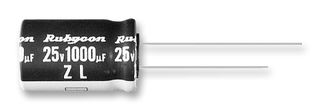
\includegraphics[scale=0.5]{capap-r.jpg}
	\caption{Condensateurs électrolytiques. (Source : datasheet du composant sur Farnell.com)}
\end{figure}

% Just here to fix rapport_prejury.tex
\end{document}